
%%%%%%%%%%%%%%%%%%%%%%%%%%%%%%%%%%%%%%%%%%%%%%%%%%%%%%%%%%%%%%%%%%%%%%%%%%%%%%
%                                                                            %
%  ************************** AVISO IMPORTANTE **************************    %
%                                                                            %
% Éste es un documento de ayuda para los autores que deseen enviar           %
% trabajos para su consideración en el Boletín de la Asociación Argentina    %
% de Astronomía.                                                             %
%                                                                            %
% Los comentarios en este archivo contienen instrucciones sobre el formato   %
% obligatorio del mismo que complementan los instructivos web y PDF.         %
% Por favor léalos.                                                          %
%                                                                            %
% No deben borrarse los comentarios en este archivo. En caso contrario,      %
% el sistema de recepción de manuscritos no permitirá el envío de su         %
% contribución. No se permite el uso de \newcommand ni definiciones          %
% particulares de cada autor.                                                %
%                                                                            %
%%%%%%%%%%%%%%%%%%%%%%%%%%%%%%%%%%%%%%%%%%%%%%%%%%%%%%%%%%%%%%%%%%%%%%%%%%%%%%

%%%%%%%%%%%%%%%%%%%%%%%%%%%%%%%%%%%%%%%%%%%%%%%%%%%%%%%%%%%%%%%%%%%%%%%%%%%%%%
%                                                                            %
%  ************************** IMPORTANT NOTICE **************************    %
%                                                                            %
%  This is a help file for authors who are preparing manuscripts to be       %
%  considered for publication in the Boletín de la Asociación Argentina      %
%  de Astronomía.                                                            %
%                                                                            %
%  The comments in this file give instructions about the manuscripts'        %
%  mandatory format that complement the instructions distributed as a PDF    %
%  and findable in the BAAA web. Please read them.                           %
%                                                                            %
%  The comments in this file must not be deleted. Otherwise, your            %
%  contribution will be rejected by the manuscript reception system.         %
%  The use of \newcommand and author definitions are forbidden.              %
%                                                                            %
%%%%%%%%%%%%%%%%%%%%%%%%%%%%%%%%%%%%%%%%%%%%%%%%%%%%%%%%%%%%%%%%%%%%%%%%%%%%%%

\documentclass[baaa]{baaa}

\usepackage[pdftex]{hyperref}
\usepackage{subfigure}
\usepackage{natbib}
\usepackage{helvet,soul}
\usepackage[font=small]{caption}

%%%%%%%%%%%%%%%%%%%%%%%%%%%%%%%%%%%%%%%%%%%%%%%%%%%%%%%%%%%%%%%%%%%%%%%%%%%%%%
%                                                                            %
%  Seleccione el idioma de su contribución: Recuerde que todos los           %
%  componentes del documento (titulo, texto, figuras, tablas, etc.)          %
%  deben estar en el mismo idioma.                                           %
%                                                                            %
%  Select the language of your contribution: Please remember that all       %
%  document parts (title, text, figures, tables, etc.) must be in the        %
%  same language.                                                            %
%                                                                            %
%  0: Castellano / Spanish                                                   %
%  1: Inglés / English                                                       %
%                                                                            %
%%%%%%%%%%%%%%%%%%%%%%%%%%%%%%%%%%%%%%%%%%%%%%%%%%%%%%%%%%%%%%%%%%%%%%%%%%%%%%

\contriblanguage{0}

%%%%%%%%%%%%%%%%%%%%%%%%%%%%%%%%%%%%%%%%%%%%%%%%%%%%%%%%%%%%%%%%%%%%%%%%%%%%%%
%                                                                            %
%  Seleccione el tipo de contribución solicitada:                            %
%                                                                            %
%  Select the requested contribution type:                                   %
%                                                                            %
%  1: Presentación mural / Poster                                            %
%  2: Presentación oral / Oral contribution                                  %
%  3: Informe invitado / Invited report                                      %
%  4: Mesa redonda / Round table                                             %
%  5: Presentación Premio Varsavsky / Varsavsky Prize contribution           %
%  6: Presentación Premio Sahade / Sahade Prize contribution                 %
%  7: Presentación Premio Sérsic / Sérsic Prize contribution                 %
%                                                                            %
%%%%%%%%%%%%%%%%%%%%%%%%%%%%%%%%%%%%%%%%%%%%%%%%%%%%%%%%%%%%%%%%%%%%%%%%%%%%%%

\contribtype{8}

%%%%%%%%%%%%%%%%%%%%%%%%%%%%%%%%%%%%%%%%%%%%%%%%%%%%%%%%%%%%%%%%%%%%%%%%%%%%%%
%                                                                            %
%  Seleccione el área temática de su contribución:                           %
%                                                                            %
%  Select the thematic area of your contribution:                            %
%                                                                            %
%  1 [AEC]:   Astrofísica Extragaláctica y Cosmología /                      %
%             Extragalactic Astrophysics and Cosmology                       %
%  2 [EG]:    Estructura Galáctica / Galactic Structure                      %
%  3 [AE]:    Astrofísica Estelar / Stellar Astrophysics                     %
%  4 [SE]:    Sistemas Estelares / Stellar Systems                           %
%  5 [ICSA]:  Instrumentación y Caracterización de Sitios Astronómicos /     %
%             Instrumentation and Astronomical Site Characterization         %
%  6 [MI]:    Medio Interestelar / Interstellar Medium                       %
%  7 [OCPAE]: Objetos Compactos y Procesos de Altas Energías /               %
%             Compact Objetcs and High-Energy Processes                      %
%  8 [SH]:    Sol y Heliosfera / Sun and Heliosphere                         %
%  9 [SSE]:   Sistemas Solar y Extrasolares / Solar and Extrasolar Systems   %
% 10 [HEDA]:  Historia, Enseñanza y Divulgación de la Astronomía /           %
%             History, Teaching and Spreading of Astronomy                   %
% 11 [O]:     Otros / Other Topics                                           %
%                                                                            %
%%%%%%%%%%%%%%%%%%%%%%%%%%%%%%%%%%%%%%%%%%%%%%%%%%%%%%%%%%%%%%%%%%%%%%%%%%%%%%

\thematicarea{99}

\title{Artículo ejemplo para publicaciones en el BAAA Vol. 61B:}
\subtitle{Instrucciones de estilo}

%%%%%%%%%%%%%%%%%%%%%%%%%%%%%%%%%%%%%%%%%%%%%%%%%%%%%%%%%%%%%%%%%%%%%%%%%%%%%%
%                                                                            %
%  Agregue un título corto para el encabezado de las páginas pares.          %
%                                                                            %
%  Add a short title to appear in the header of even pages.                  %
%                                                                            %
%%%%%%%%%%%%%%%%%%%%%%%%%%%%%%%%%%%%%%%%%%%%%%%%%%%%%%%%%%%%%%%%%%%%%%%%%%%%%%

\titlerunning{Macro BAAA61B con instrucciones de estilo}

%%%%%%%%%%%%%%%%%%%%%%%%%%%%%%%%%%%%%%%%%%%%%%%%%%%%%%%%%%%%%%%%%%%%%%%%%%%%%%
%                                                                            %
%  Lista de autores. Los nombres de los autores deben estar separados por    %
%  comas, y deben tener el formato A.E. Autor (iniciales apellido(s); sin    %
%  coma entre apellido e iniciales ni espacios entre las iniciales).         %
%                                                                            %
%  Author list. Authors' names must be separated by commas, and stick to     %
%  the format A.E. Author (initials Family name -neither commas between      %
%  name and the initials nor blanks between the initials).                   %
%                                                                            %
%%%%%%%%%%%%%%%%%%%%%%%%%%%%%%%%%%%%%%%%%%%%%%%%%%%%%%%%%%%%%%%%%%%%%%%%%%%%%%

\author{A.M. Vásquez\inst{1}, P. Benaglia\inst{2}, F.A. Iglesias\inst{3}, \& M.A. Sgr\'o\inst{4}}
\authorrunning{Vásquez et al.}

%%%%%%%%%%%%%%%%%%%%%%%%%%%%%%%%%%%%%%%%%%%%%%%%%%%%%%%%%%%%%%%%%%%%%%%%%%%%%%
%                                                                            %
% Por favor provea una dirección de e-mail de contacto para los lectores.    %
%                                                                            %
% Please provide a contact e-mail address for the readers.                   %
%                                                                            %
%%%%%%%%%%%%%%%%%%%%%%%%%%%%%%%%%%%%%%%%%%%%%%%%%%%%%%%%%%%%%%%%%%%%%%%%%%%%%%

\contact{editor.baaa@gmail.com}

\institute{
Insituto de Astronomía y Física del Espacio, CONICET--UBA, Argentina \and
Instituto Argentino de Radioastronomía, CONICET-CICPBA, Argentina \and
Grupo de Estudios Atmosf\'ericos y Ambientales, UTN-FRM y CONICET, Argentina \and
Instituto de Astronom\'ia Te\'orica y Experimental, CONICET--UNC, Argentina
}

%%%%%%%%%%%%%%%%%%%%%%%%%%%%%%%%%%%%%%%%%%%%%%%%%%%%%%%%%%%%%%%%%%%%%%%%%%%%%%
%                                                                            %
%  El resumen y el abstract son ambos obligatorios, independientemente del   %
%  lenguaje elegido.                                                         %
%                                                                            %
%  The Resumen and the abstract are both mandatory, regardless of the chosen %
%  language.                                                                 %
%                                                                            %
%%%%%%%%%%%%%%%%%%%%%%%%%%%%%%%%%%%%%%%%%%%%%%%%%%%%%%%%%%%%%%%%%%%%%%%%%%%%%%

\resumen{
Esta es una guía para la preparación de artículos a enviarse al \textit{Boletín de la Asociación Argentina de Astronomía} (BAAA), que además sirve de macro para la edición 61B. El presente será el único formato aceptado de los artículos recibidos por los editores. Su envío deberá hacerse exclusivamente mediante el Sistema de Gestión de Manuscritos.}

\abstract{
This is a guide for authors who are preparing papers for the \textit{Boletín de la Asociación Argentina de Astronomía} (BAAA), intended also as a macro for the Volume 61B. This will be the only format accepted for article submission and has to be implemented through the Manuscript Management System exclusively.
}

%%%%%%%%%%%%%%%%%%%%%%%%%%%%%%%%%%%%%%%%%%%%%%%%%%%%%%%%%%%%%%%%%%%%%%%%%%%%%%
%                                                                            %
%  Seleccione las palabras clave que describen su contribución. Las mismas   %
%  son obligatorias, y deben tomarse de la lista de la American Astronomical %
%  Society (AAS), que se encuentra en la página web indicada abajo.          %
%                                                                            %
%  Select the keywords that describe your contribution. They are mandatory,  %
%  and must be taken from the list of the American Astronomical Society      %
%  (AAS), which is available at the webpage quoted below.                    %
%                                                                            %
%  https://aas.org/authors/astronomical-subject-keywords-update-august-2013  %
%                                                                            %
%%%%%%%%%%%%%%%%%%%%%%%%%%%%%%%%%%%%%%%%%%%%%%%%%%%%%%%%%%%%%%%%%%%%%%%%%%%%%%

\keywords{editorials, notices --- miscellaneous}

\begin{document}

\maketitle

\section{Introducción}
\label{S_intro}

La 61a reunión anual de la Asociación Argentina de Astronomía se desarrolló del 16 al 20 de septiembre de 2019 en la ciudad de Viedma, Río Negro, Argentina. Durante la misma se expusieron 68 trabajos en forma de presentación mural y 55 trabajos en forma de presentación oral, incluyendo doce charlas plenarias y una correspondiente al premio ``José Luis Sérsic'' al Investigador Consolidado (otorgado por la AAA). Asimismo, se desarrollaron una mesa redonda, una asamblea extra\-ordinaria y otra ordinaria. Los invitamos cordialmente ahora a remitir sus contribuciones en forma escrita para que las mismas puedan ser consideradas para su publicación en el Boletín No. 61B de la AAA.

El Comité Editorial del presente volumen está integrado por Alberto M. Vásquez como Editor en Jefe, Francisco A. Iglesias como Secretario Editorial y Mario A. Sgró como Técnico Editorial. El Editor Invitado es Paula Benaglia, quién se desempeñó como Presidente del Comité Organizador Científico de la reu\-nión.

Recordamos que el Reglamento de Publicaciones\footnote{\url{http:// www.astronomiaargentina.org.ar/uploads/docs/reglamento_de_publicaciones.pdf}} de la Asociación regula el alcance del BAAA en sus artículos 2 al 7.

Esperamos que todas las contribuciones presentadas durante la reunión sean publicadas en la próxima edición del Boletín. Particularmente importantes serán los artículos correspondientes a las charlas invitadas dado el carácter de revisión que deben tener los mismos sobre áreas específicas. Excepto estos últimos, y los co\-rres\-pon\-dien\-tes a premios y mesas redondas, todos los trabajos que se envíen serán revisados por árbitros asignados por los editores. Los árbitros deberán constatar si el trabajo presentado tiene elementos originales. Esto debe tenerse en cuenta principalmente en las contribuciones derivadas de presentaciones en la reunión sobre artículos ya publicados. En tales casos, se requerirá que el texto y las figuras  presenten información adicional a dichas publicaciones. Los trabajos aceptados formarán parte de la base de publicaciones del ADS.
                                                                   
Agradecemos desde ya a todos el envío de sus contribuciones en tiempo y forma, ayudando a lograr que la edición 61B de la única publicación de astronomía profesional de la Argentina se publique lo antes posible.

\section{Instrucciones}

Los manuscritos a remitir podrán ser escritos en cas\-te\-lla\-no o en inglés, a elección del autor. En cualquier caso deberán incluir un resumen en ambas lenguas. Existen dos categorías de trabajos: cortos de tres páginas de extensión y largos de siete páginas. Los cortos corresponden a Comunicación Oral o Mural, los largos co\-rres\-pon\-den a Informe Invitado, Mesa Redonda o Premio. Se adjuntan al presente archivo los nuevos macros de estilo del BAAA e instrucciones para los autores, estas últimas en forma de un archivo ejemplo: {\tt articulo.tex}. Estos archivos pueden también bajarse de la página Web del Sistema de Gestión de Manuscritos  (SiGMa: \url{http://sigma.astronomiaargentina.org.ar/}), a través de la cual se realiza la carga de contribuciones y su seguimiento durante la etapa de revisión. El archivo {\tt articulo.tex} puede también encontrarse en el sistema de edición en línea de archivos \LaTeX{} \emph{Overleaf} (\url{https://www.overleaf.com/}) como el ``template" ti\-tu\-la\-do \emph{Boletín Asociación Argentina de Astronomía}.

Una vez abierto el plazo de recepción de contribuciones (anunciado oportunamente), la recepción de trabajos correspondientes a comunicación oral o mural se extiende hasta el día 3 de noviembre de 2019 (inclusive). Las contribuciones tipo informe invitado, mesa redonda o premio se recibirán hasta el 1ro de diciembre de 2019 (inclusive). La recepción finalizará automáticamente en dichos plazos, por lo que no se admitirán contribuciones que se reciban más allá de las fechas indicadas.

Para el envío de trabajos, los autores deberán preparar el archivo de texto siguiendo
el formato del presente instructivo (archivo ``tex'').  Las figuras deberán estar en alguno de los siguientes formatos: ``pdf'', ``jpg'' o ``png''. La bibliografía tendrá que ser preparada según el estándar \textsc{bibtex}  (ver sección~\ref{ref}).

Para la preparación de manuscritos se solicita: 

\begin{itemize}
   \item Utilizar este macro exclusivamente; no serán aceptados trabajos compilados con macros viejos.
   \item No agregar definiciones propias en \LaTeX{}, ya que los encabezamientos individuales son ignorados en la compilación general del volumen.
   \item Emplear el mismo idioma para texto y figuras.
   \item Leer cuidadosamente la guía de estilo. 
\end{itemize}

No serán admitidas contribuciones que excedan el límite de páginas especificado para cada modalidad de trabajo, aún después de introducir las correcciones. Queda a cargo de los autores hacer los ajustes de extensión que resulten necesarios.

\section{Guía de estilo para el BAAA}

A continuación reproducimos algunos lineamientos del manual de estilo. Esta lista no es exhaustiva, pero contiene algunos aspectos básicos útiles para preparar la contribución. El manual completo está disponible en la web del SiGMa (\url{http://sigma.astronomiaargentina.org.ar/docs/SGM_docs_v01/Surf/M0SM5.html}) y recomendamos leerlo atentamente para preparar el manuscrito. Agradecemos a los autores este trabajo adicional, que hará posible una edición más rápida del volumen.

\subsection{Palabras clave: $Keywords$}

La inclusión de palabras clave, en inglés, es obligatoria. El delimitador de palabras clave es el triple guión. Para la selección de palabras utilizar la \href{http://www.aanda.org/author-information/acceptance-stage?task=view&id=170}{lista de la revista Astronomy \& Astrophysics}.\,\footnote{\url{http://www.aanda.org/author-information/acceptance-stage?task=view&id=170}}

\subsection{Texto}

Destacamos a continuación algunos puntos del manual de estilo.

\begin{itemize}
  \item Las unidades van separadas de la magnitud por un espacio inseparable ($\sim$) y se escriben con tipografía de texto normal (no cursiva). No llevan punto de abreviación; ej.: mag, km (no: mag., km.).
  \item Para separar parte entera de decimal en números utilizar un punto (no coma).
  \item Para grandes números, separar en miles usando el espacio reducido; ej.: $1\,000\,000$ (\verb+$1\,000\,000$+).
  \item Las abreviaturas van en mayúsculas; ej.: UV, IR, R-X.
  \item Para abreviar ``versus'' utilizar ``vs.'' y no ``Vs.''.
  \item Las comillas son dobles y no simples; ej.: ``palabra'', no `palabra'.
  \item Las llamadas a figuras y tablas comienzan con mayúscula si van seguidas del número correspon\-dien\-te; ej.: Fig., Ec. o Sec. Tabla, en cambio, con pa\-la\-bra completa.
  \item Si el texto está escrito en castellano, no utilizar el idioma inglés para términos o palabras que tengan  su correspondiente traducción en castellano. Solo cuando la inclusión de una palabra en inglés es, a juicio del autor, absolutamente inevitable, incluir dicha palabra en {\em cursiva}.
  \item Especies atómicas se indican, por ejemplo, \verb|He {\sc ii}| (He {\sc ii}).
% \item No agregar punto final al título.
% \item Autores: Iniciales del nombre y luego el apellido. Si se envían varios artículos, revisar que el nombre aparezca igual en todos ellos, especialmente en apellidos dobles y con guiones.
% \item El último autor se separa con ``\&'' del resto.
  \item No están permitidas las referencias en el resumen y $abstract$.
% \item Los títulos, contenido y anotaciones de las figuras deben estar en el mismo idioma, salvo que se cite como extraído de otro trabajo.
  \item No está permitido el uso de comandos que mo\-di\-fiquen las propiedades del texto, como $small$, $scriptsize$, etc. Téngase en cuenta esto especialmente en tablas, figuras y leyendas.
\end{itemize}

Si algunos casos no están incluidos en el manual de estilo del BAAA, se solicita seguir el estilo de la revista Astronomy \& Astrophysics\footnote{\url{http://www.aanda.org/author-information/latex-issues/typography}}.

\subsection{Ecuaciones y símbolos matemáticos}

Las ecuaciones van numeradas (para su correcta identificación y referencia): usar \verb|\begin{equation}| y \verb|\end{equation}| o similares ($align$, etc.). Las ecuaciones en modo $display$ deben llevar al final la puntuación gramatical correspondiente, como parte de la frase en la que están insertas. En particular, los vectores deben ir en ``negrita'' (con \verb+\mathbf{}+) y no con ``flechita''.

\subsection{Tablas}

En las tablas se debe incluir cuatro líneas: dos superiores, una inferior y una que separa el encabezado. Se pueden confeccionar tablas de una columna (\verb|\begin{table}|) o de todo el ancho de la página (\verb|\begin{table*}|). Las tablas no deben sobrepasar los márgenes establecidos para el texto (ver Tabla \ref{tabla1}), y no se pueden usar modificadores del tamaño de texto.

\begin{table}[!t]
\centering
\caption{Ejemplo de tabla {\bf no aceptable} ya que excede el margen de la columna de texto.}
\begin{tabular}{lccc}
\hline\hline\noalign{\smallskip}
Date & Coronal $H_r$ & Diff. rot. $H_r$& Mag. clouds $H_r$\\
& 10$^{42}$ Mx$^{2}$& 10$^{42}$ Mx$^{2}$ & 10$^{42}$ Mx$^{2}$ \\
\hline\noalign{\smallskip}
07 July  &  -- & (2) & [16,64]\\
03 August& [5,11]& 3 & [10,40]\\
30 August & [17,23] & 3& [4,16]\\
25 September & [9,12] & 1 & [10,40]\\
\hline
\end{tabular}
\label{tabla1}
\end{table}
 
\begin{table}[!t]
\centering
\caption{Una posible solución al problema de exceso del margen mostrado en la Tabla~\ref{tabla1}.}
\begin{tabular}{lccc}
\hline\hline\noalign{\smallskip}
\!\!Date & \!\!\!\!Coronal $H_r$ & \!\!\!\!Diff. rot. $H_r$& \!\!\!\!Mag. clouds $H_r$\!\!\!\!\\
& \!\!\!\!10$^{42}$ Mx$^{2}$& \!\!\!\!10$^{42}$ Mx$^{2}$ & \!\!\!\!10$^{42}$ Mx$^{2}$ \\
\hline\noalign{\smallskip}
\!\!07 July  &  -- & (2) & [16,64]\\
\!\!03 August& [5,11]& 3 & [10,40]\\
\!\!30 August & [17,23] & 3& [4,16]\\
\!\!25 September & [9,12] & 1 & [10,40]\\
\hline
\end{tabular}
\end{table}

\subsection{Figuras}

Las figuras deberán prepararse en formatos ``jpg'', ``png'' o ``pdf'', siendo este último el de preferencia.

Al preparar figuras deberá tenerse en cuenta que las mismas deben incluir todos los elementos que posibiliten su lectura, tales como escalas y nombres de los ejes, códigos de líneas, símbolos, etc. El lenguaje de las palabras en los gráficos debe ser el mismo que el lenguaje del resto del artículo. Si bien la impresión del BAAA se hace en escala de grises, la mayor distribución del mismo es electrónica, por lo que es posible realizar figuras a color, siempre que no se pierda información cuando se visualiza en escala de grises.

Es recomendable tener en cuenta ciertos aspectos para asegurar la legibilidad y el impacto deseado. La correcta presentación de las figuras se puede resumir a dos puntos: el tamaño del texto y la resolución. Se su\-gie\-re que las letras tengan el mismo tamaño que en el texto (ver Fig.~\ref{F_letras}).

Para figuras que hayan sido tomadas de otras pu\-bli\-ca\-cio\-nes, es necesario contar con el permiso de reproducción respectivo.

%%%%%%%%%%%%%%%%%%%%%%%%%%%%%%%%%%%%%%%%%%%%%%%%%%%%%%%%%%%%%%%%%%%%%%%%%%%%%%
%                                                                            %
% Para figuras de dos columnas use \begin{figure*} ... \end{figure*}         %
%                                                                            %
%%%%%%%%%%%%%%%%%%%%%%%%%%%%%%%%%%%%%%%%%%%%%%%%%%%%%%%%%%%%%%%%%%%%%%%%%%%%%%

\begin{figure}[!t]
  \centering
  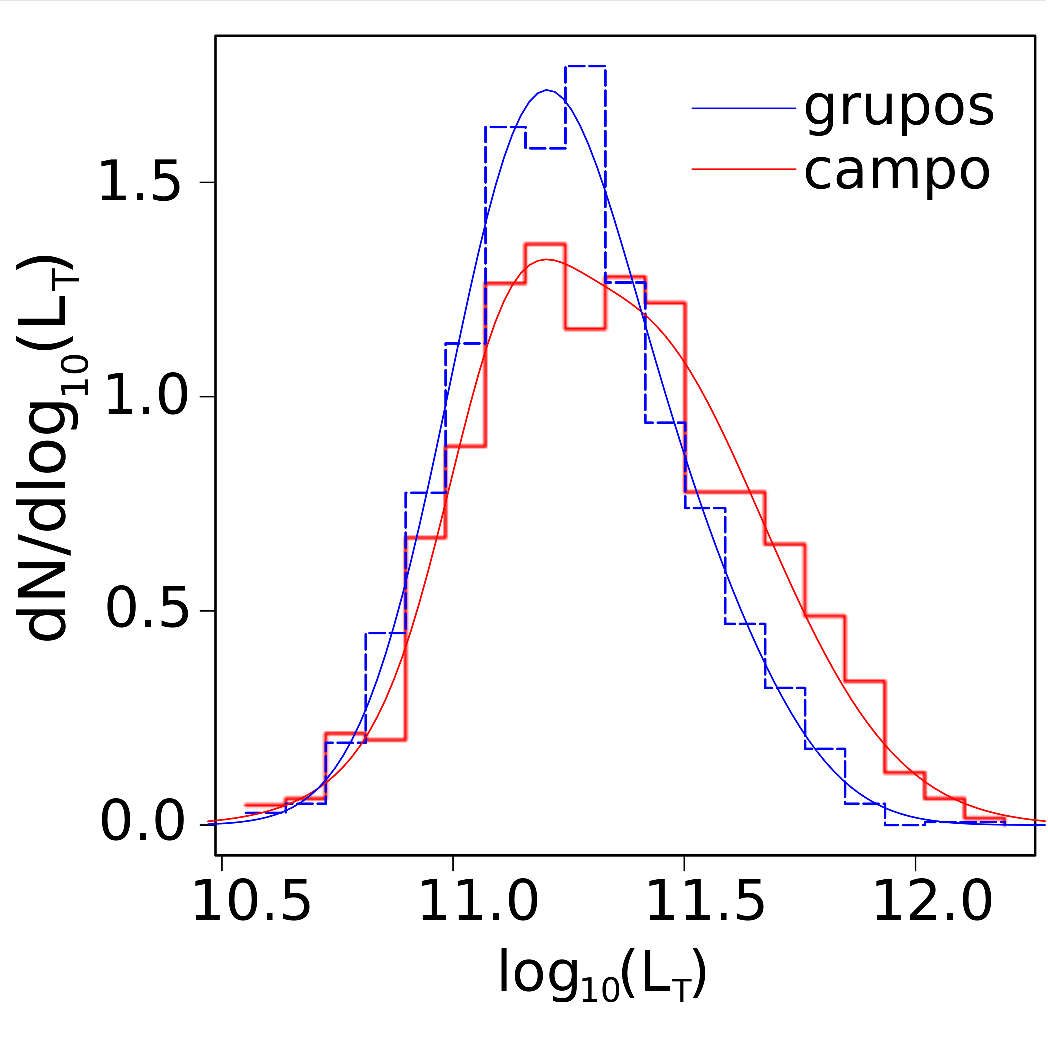
\includegraphics[width=0.36\textwidth]{ejemplo_fig01.pdf}
  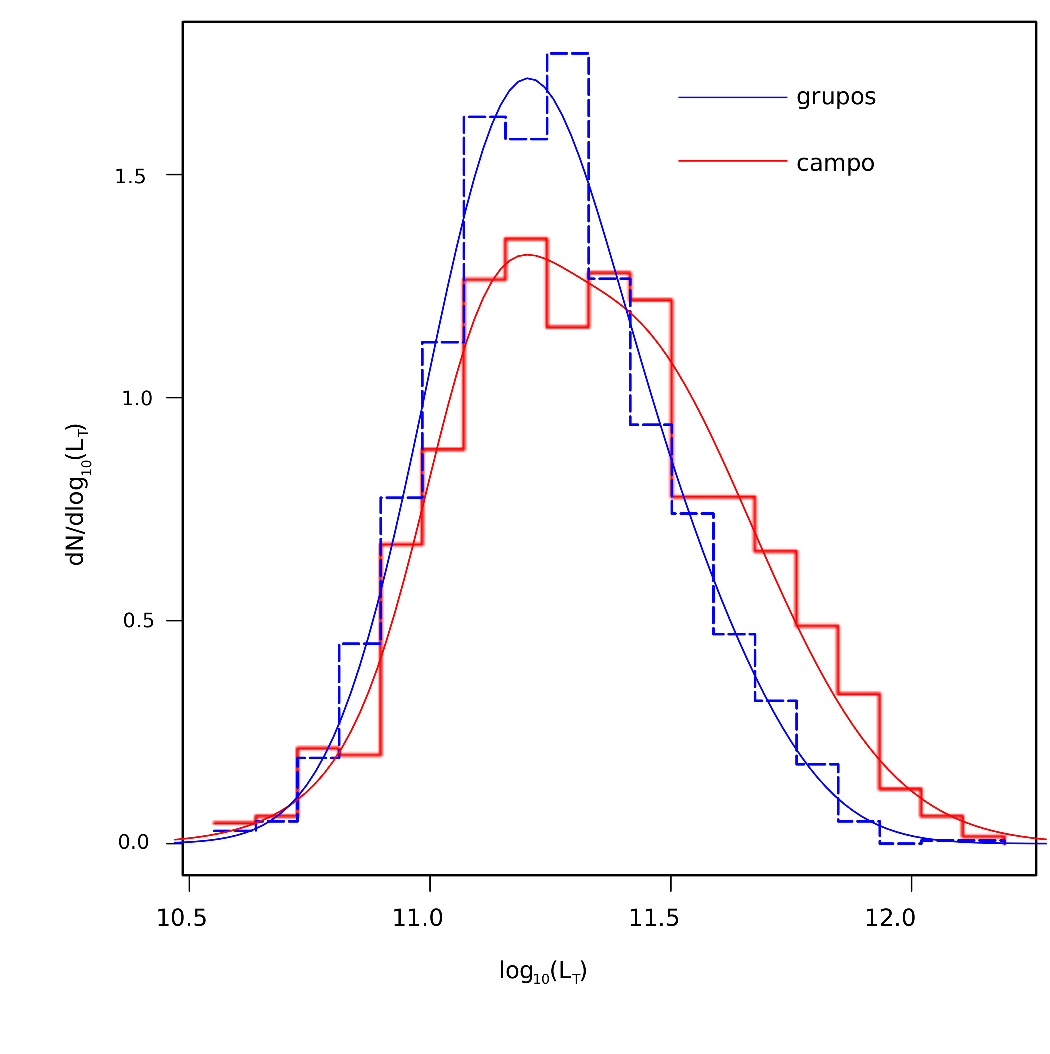
\includegraphics[width=0.36\textwidth]{ejemplo_fig02.pdf}
  \caption{Panel superior: Ejemplo de figura con letras muy grandes.
           Panel inferior: Ejemplo con letras muy pequeñas.
}
  \label{F_letras}
\end{figure}

\subsection{Referencias cruzadas}
\label{ref}

Es recomendable utilizar referencias cruzadas al escribir un artículo. Este método permite hacer dinámico el documento, es decir, navegar entre tablas, figuras y secciones si se utiliza el software adecuado (Acrobat Reader, etc). Por ejemplo, se puede citar la introducción (Sec.~\ref{S_intro}), una figura (Fig.~\ref{F_letras}), o una tabla (Tabla~\ref{tabla1}).

Debe incorporarse el uso de {\sc bibtex}, la herramienta desarrollada para escribir y procesar listas de referencias. De esta forma, durante la compilación, \LaTeX{} toma del archivo de referencias solamente las que fueron citadas en el texto. El estilo de las referencias se aplica automáticamente a través de un archivo de estilo (baaa.bst).

{\sc bibtex} es muy utilizado por casi todas las editoriales de revistas científicas, y en los últimos años su uso se ha popularizado gracias a programas de administración de listas bibliográficas, que generan los archivos necesarios (.bib) de manera muy sencilla.

La base de datos del ADS contiene las entradas de {\sc bibtex}  para todos los artículos.  Se puede acceder a ellas mediante el enlace ``{\em Bibtex entry for this abstract}''.

Las referencias así generadas tendrán la forma co\-rrec\-ta para un autor \citep{hubble_expansion_1929}, dos autores \citep{penzias_cmb_1965}, tres autores \citep{navarro_NFW_1997} y muchos autores \citep{riess_SN1a_1998}, \citep{Planck_2016}. Se proporciona un archivo de ejemplo (biblio.bib).

\begin{acknowledgement}
Los agradecimientos deben agregarse usando el entorno correspondiente (\texttt{acknowledgement}). Agradecemos a todos los miembros de los Comités Organizadores Local y Científico por su activa participación que permitió llevar a cabo una exitosa reunión. También se agradece a los participantes por contribuir a que este congreso se haya enriquecido con muchos trabajos valiosos y animadas discusiones.
\end{acknowledgement}

%%%%%%%%%%%%%%%%%%%%%%%%%%%%%%%%%%%%%%%%%%%%%%%%%%%%%%%%%%%%%%%%%%%%%%%%%%%%%%
%                                                                            %
%  Por favor no modifique las líneas de la bibliografía, salvo el nombre     %
%  el archivo de Bibtex con la lista de citas (sin la extensión .BIB)        %
%                                                                            %
%  Please do not modify the following lines, except the name of the Bibtex   %
%  file (whithout the .BIB extension)                                        %
%                                                                            %
%%%%%%%%%%%%%%%%%%%%%%%%%%%%%%%%%%%%%%%%%%%%%%%%%%%%%%%%%%%%%%%%%%%%%%%%%%%%%% 

\bibliographystyle{baaa}
\small
\bibliography{bibliografia}
 
\end{document}
